
\section{Simulation}\label{sec:simulation}
This section examples four main challenges for pose and torque control of an object, arranged in increasing difficulty.  Each task uses a PD controller that uses the mean position and mean velocity to regulate the swarm's mean position,  as in \cite{ShahrokhiIROS2015}. The control input is the global force applied to each robot:
\begin{align}
u_x &= K_{p}(goal_x - \bar{x}) + K_{d}(0-\bar{v}_x) \nonumber\\
u_y &= K_{p}(goal_y  - \bar{y}) + K_{d}(0-\bar{v}_y)  \label{eq:PDcontrolPosition}
\end{align}
here $K_{p}$ is the proportional gain, and $K_{d}$ is the derivative gain.  
The swarm's average position is $(\bar{x},\bar{y})$ and mean velocity is $(\bar{v}_x,\bar{v}_y)$.  
Each task uses a different algorithm to select the swarm's goal position $(goal_x,goal_y)$.

\paragraph{Pure torque control} 
An object with a pivot point can rotate, but not translate. A door is a common example of an object with a pivot. A door can have an angular velocity but cannot translate. 
 If there was only one robot touching the object, the robot should push at the point which maximizes the moment arm, at the extreme end of the object furthest from the pivot point.
The optimal pushing location provides the maximum force, because it maximizes  $r$ in \eqref{eq:torque}.
However, given a swarm of robots, maximizing $r$ is no longer the optimal solution.  
If the swarm hit the object with its mean position at the extreme edge, half of the robots will miss the object and  the swarm will be torn apart.
Because few robots remain,  the force is significantly decreased and torque is not maximized.
 In our simulation, the swarm apples torque until the swarm's mean position is beyond the object.  At this point, the swarm will be regathered in a corner, a time consuming task. 
 The key parameter of interest for a hinged door of length $L$ is $C/L$, where $C$ is the position along the door where the mean of the swarm will push.  The swarm is directed toward 
 
\begin{align}\nonumber
goal_x &= O_x + C \sin(O_{\theta}- \theta_{goal}) \\
goal_y &= O_y + C \cos(O_{\theta}- \theta_{goal})  \label{eq:TorqueControl}
\end{align}

 Fig. \ref{fig:LFig} illustrates how different values of $C$ result in different rates of turning. These simulations tested $C = \{1/2, 3/4, 5/8, 1\}L$  The fastest turning rates occurred with  $C =  5/8L$. 



\begin{figure}
\begin{center}
	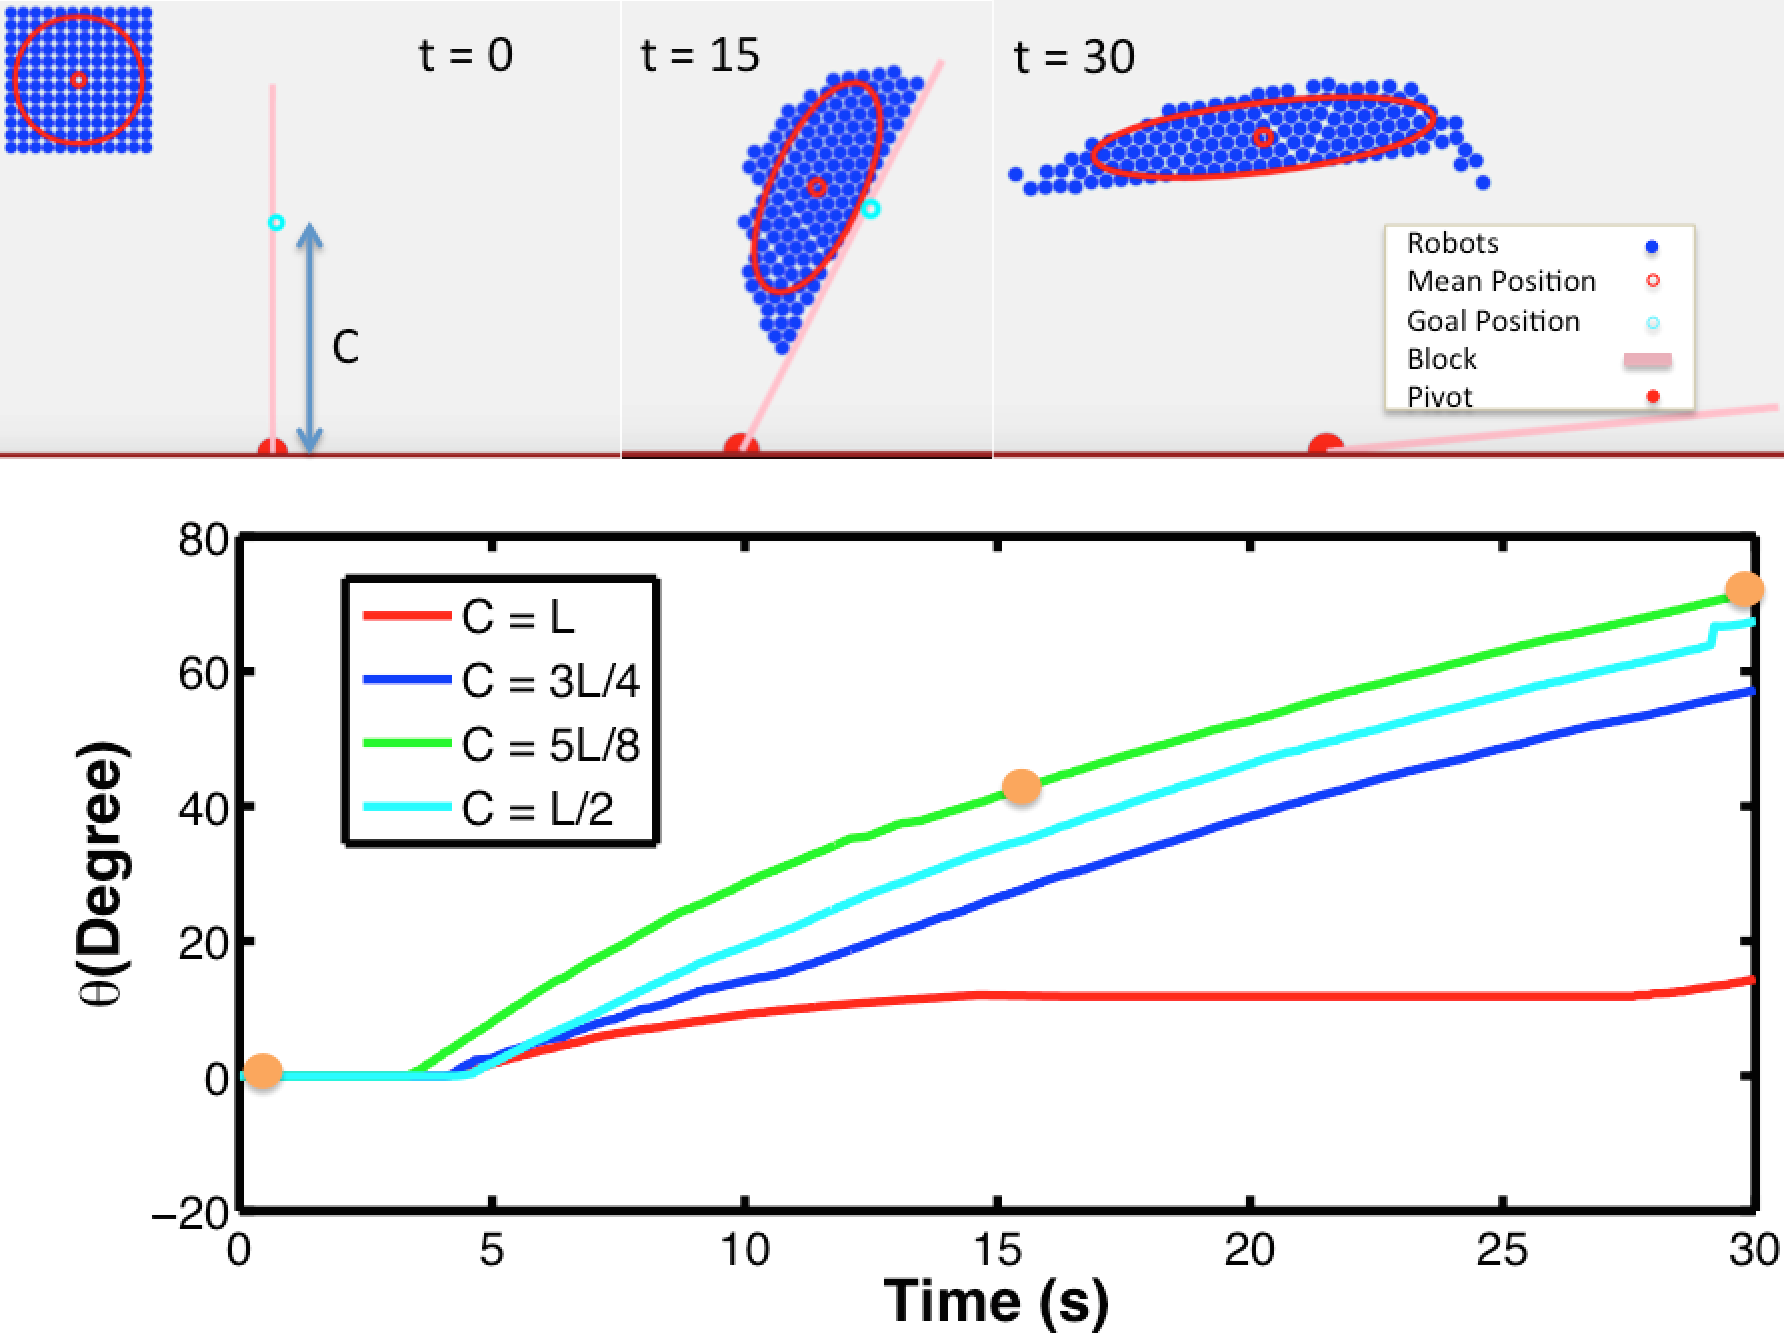
\includegraphics[width=\columnwidth]{LFig.png}
\end{center}
\vspace{-1em}
\caption{\label{fig:LFig}
Simulation results from a swarm applying force to a hinged door. 
The swarm mean is steered toward a point $C$ units along the object from the pivot point. The red dashed line indicates the times that the swarm was in variance control mode.
 Simulation used 144 robots of diameter $XX$ with a standard deviation of less than $1.5$ m and an object length of $6$ m.
}
\vspace{-1em}
\end{figure}


\paragraph{Orientation of the object}
These simulations used a uniform density rectangle as the object. This object was 30$\times$ larger than the robots.
Using the pure torque control discussed in the previous paragraph, the orientation of the object can be controlled by applying force. 
The rectangular object is not pivoted, so it moves in addition to rotating. 
 The swarm still may split into multiple components.
  We use the hysteresis variance control from \cite{ShahrokhiIROS2015}  to gather the swarm when its variance grows too large. 
  The following control law chooses a goal position to regulate the orientation of the object.  In the following equation, $O_{\theta}$ is the orientation of the object's major axis. The object COM is at $(O_x,O_y)$.

Let $\theta_O$ = the orientation of the object's major axis, measured from the world $x$-axis.
\begin{align}\nonumber
goal_x = O_x +  K_{orient}  ( \theta_O - \theta_{desired} ) \cos(\theta_O) \\
goal_y = O_y +  K_{orient}  ( \theta_O - \theta_{desired} ) \sin(\theta_O)
\end{align}
Here $K_{orient}$ is a positive gain on the control input.  


\begin{figure}
\begin{center}
	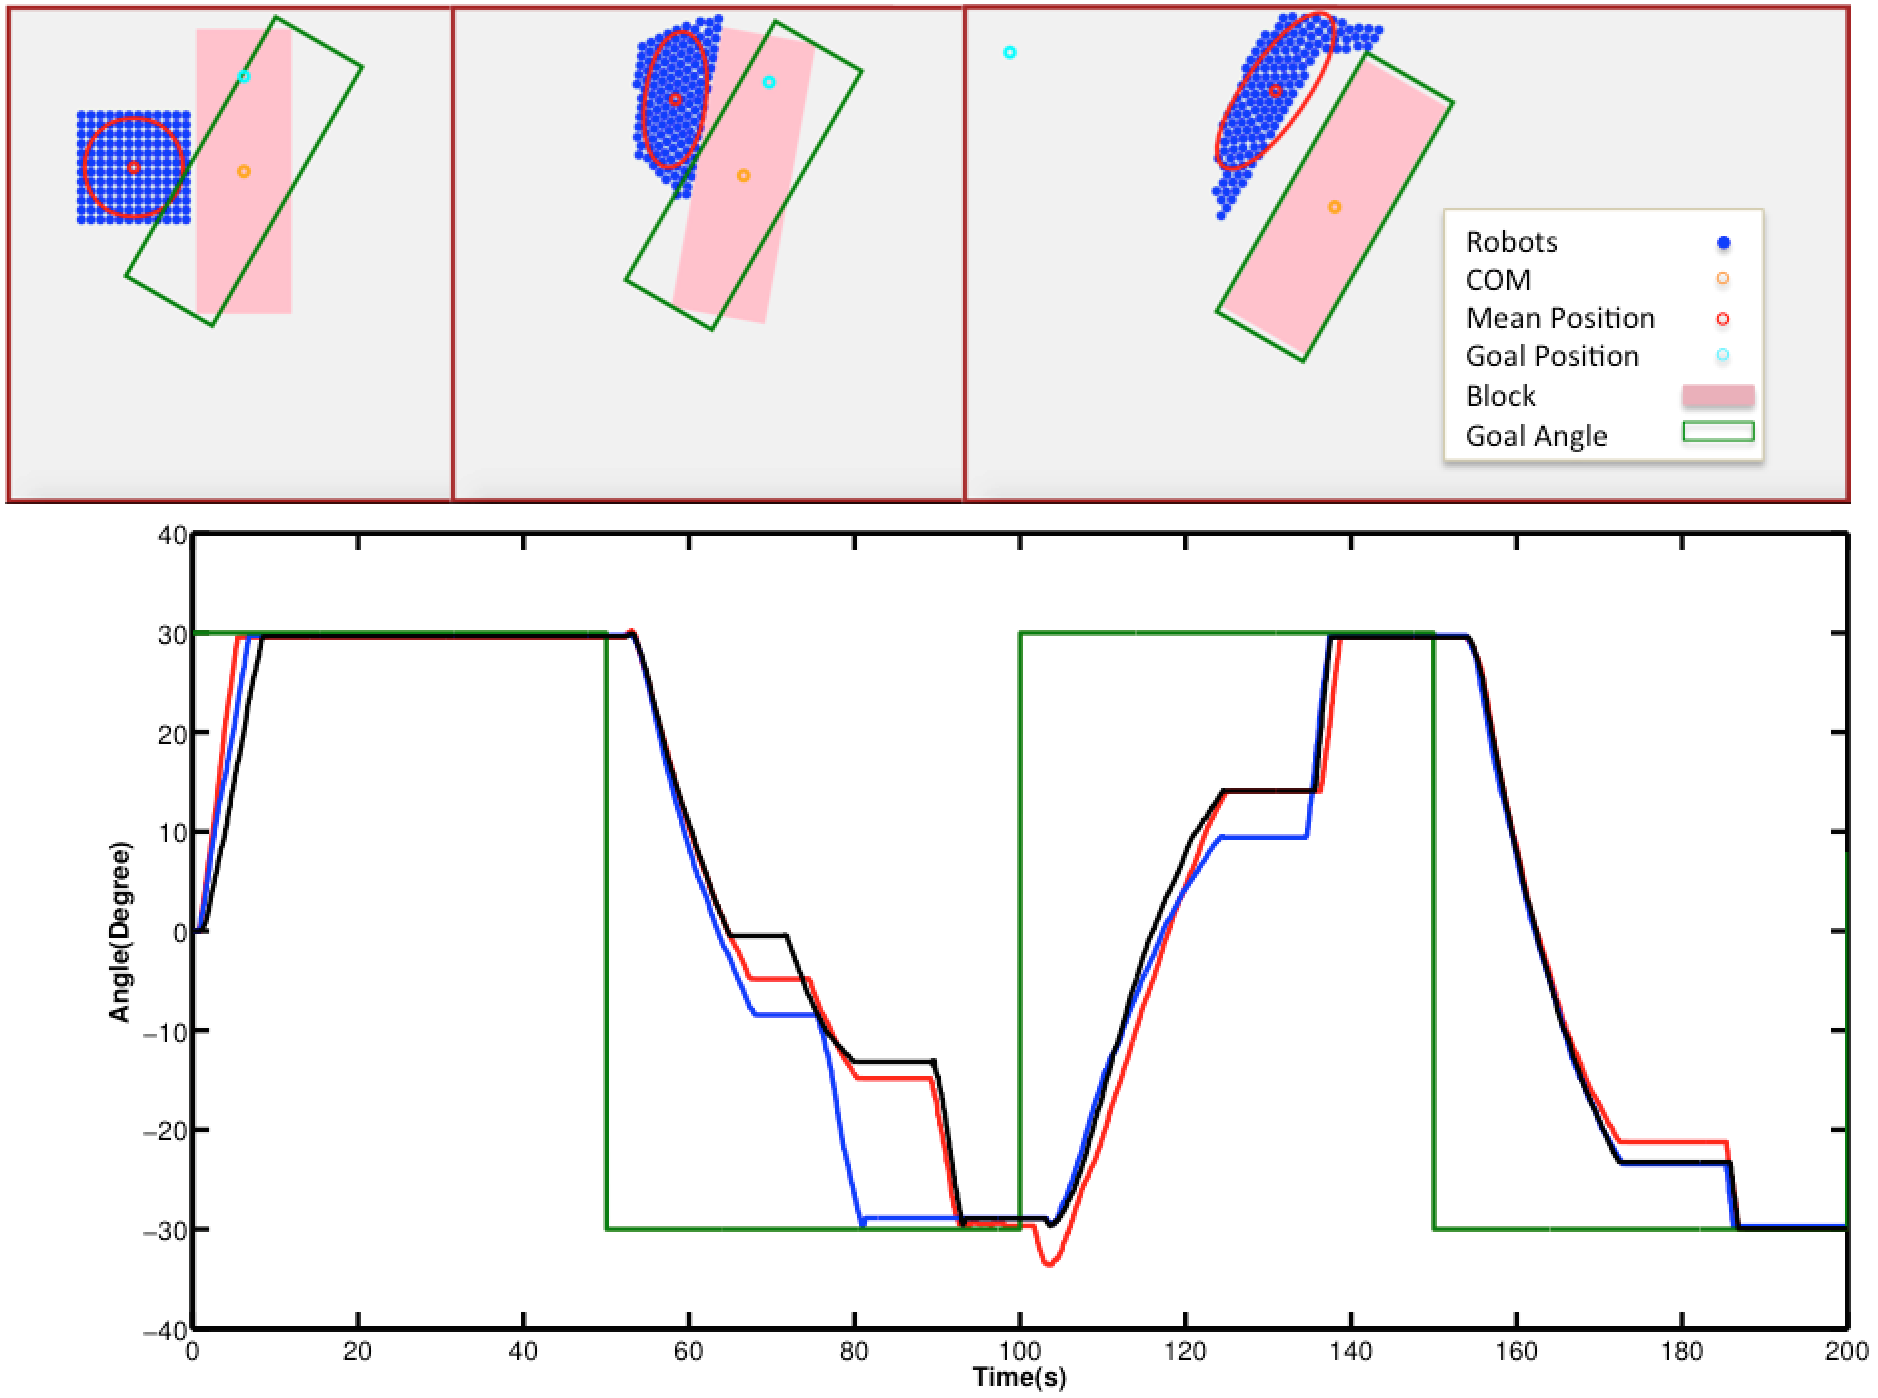
\includegraphics[width=\columnwidth]{Orientation.png}
\end{center}
\vspace{-1em}
\caption{\label{fig:OrientCont}
Plot demonstrating  orientation control of a rectangular object. The green line is the goal orientation.   When the plot traces are constant the swarm is no longer pushing the object and instead is being regathered in a corner of the workspace until the variance is below a desired threshold. 
}
\vspace{-1em}
\end{figure}

Fig. \ref{fig:OrientCont} illustrates this controller with different starting positions. When the plot traces are constant the swarm is no longer pushing the object and instead is being regathered in a corner of the workspace. 

\paragraph{Translation straight while regulating orientation of the object} \label{para:PureTranslation}

When the total force is applied perpendicular to the object and in line with the center of mass, according to Eq. \ref{eq:torque} there will be no torque. 
The following goal position for the mean position of the swarm regulates the object's orientation using $\Delta \theta$ for proportional feedback  to determine where to apply force.
$\Delta_\theta = goal_\theta - O_\theta$ is the difference between the goal angle and the current object angle.
 $K_\tau$ is a constant and $(O_x,O_y)$ is the position of the object's COM.
\begin{align}
goal_x &= O_x \nonumber \\
goal_y &= K_\tau \Delta\theta + O_y
\end{align}

 Fig. \ref{fig:Straight} shows how $\Delta \theta$ converges to zero with different initial configurations of the swarm. When the swam is above or below of the object the swarm applies a torque to the object.
 
 
\begin{figure}
\begin{center}
	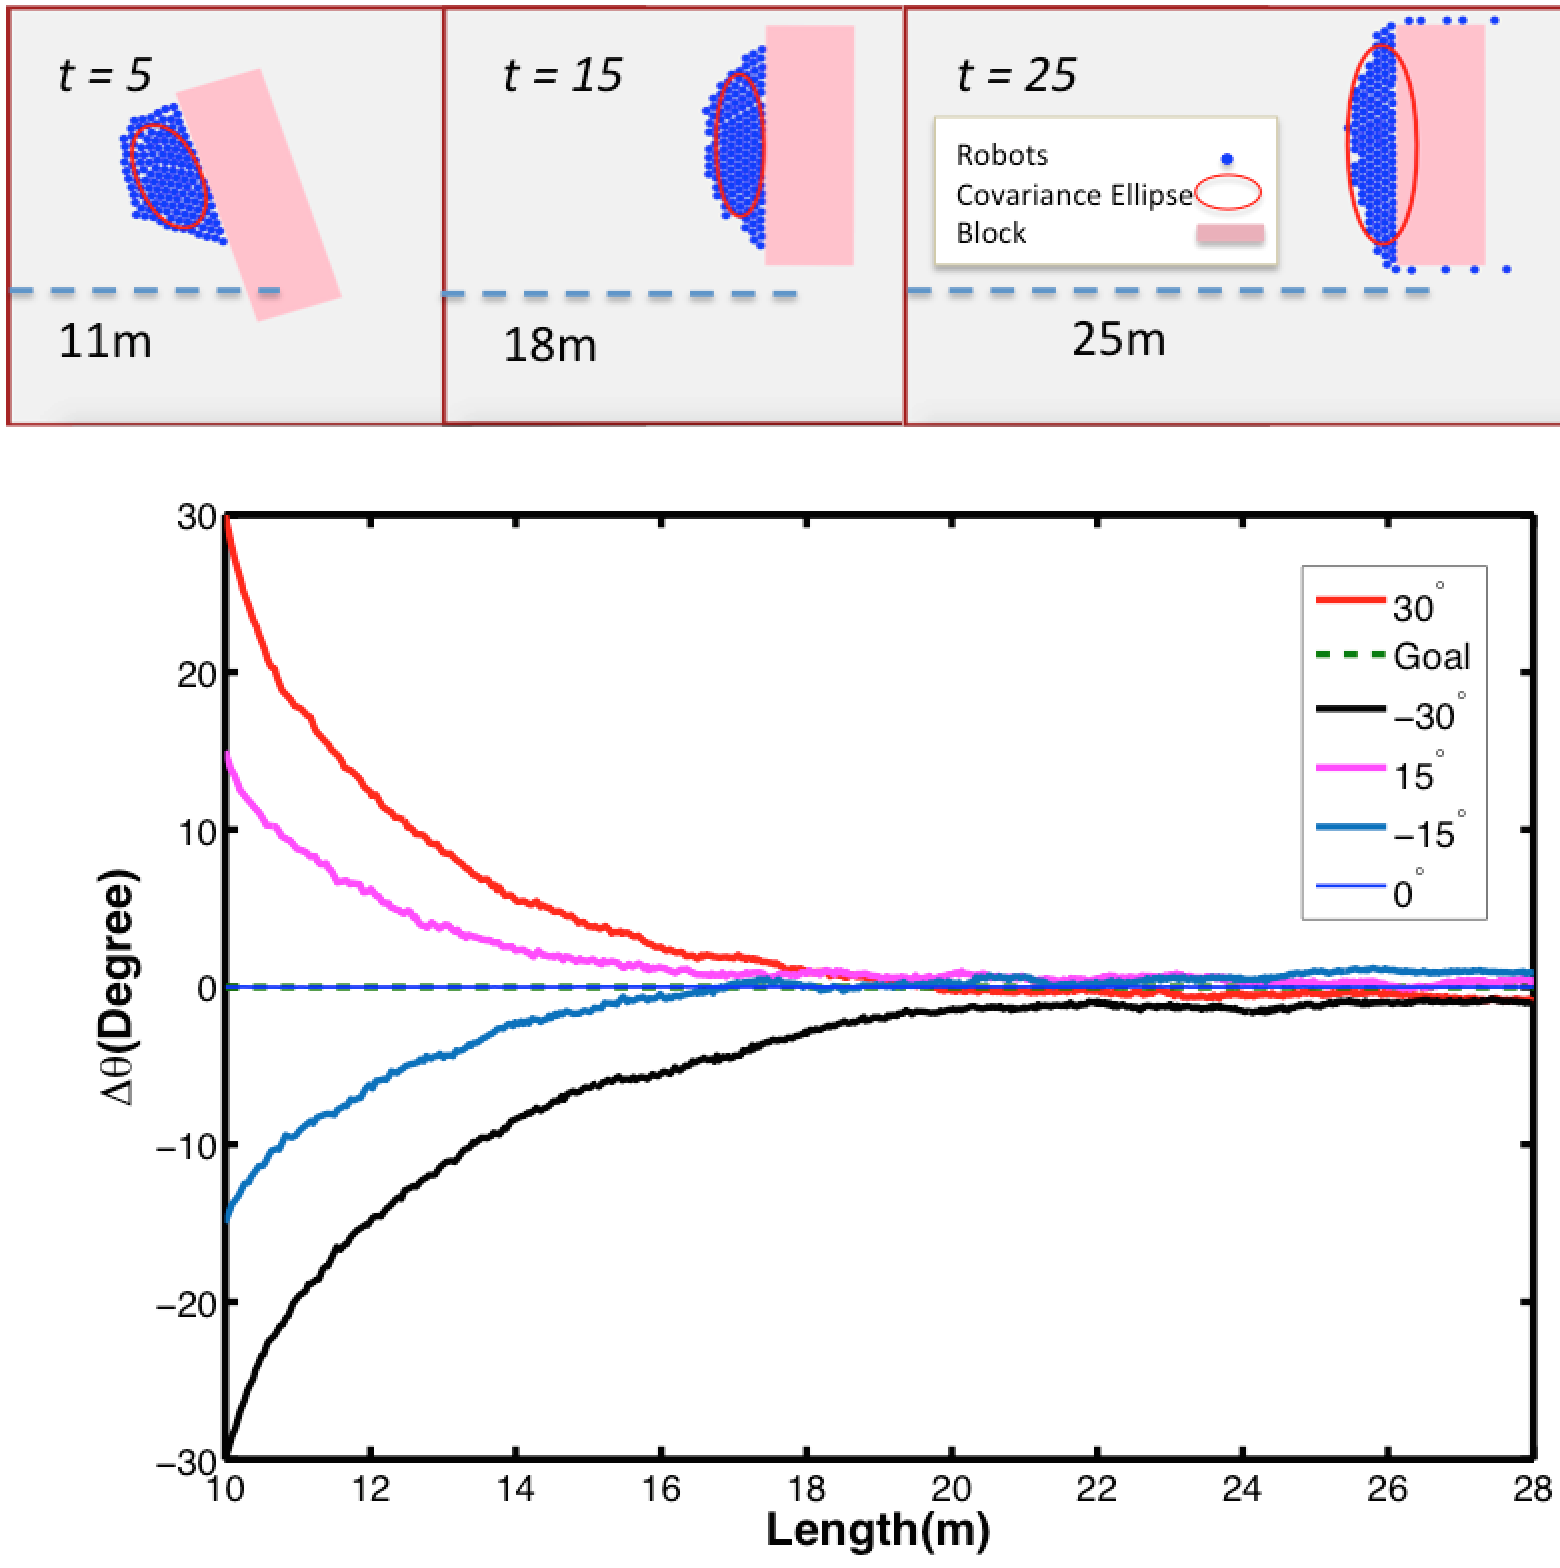
\includegraphics[width=\columnwidth]{Straight.png}
\end{center}
\vspace{-1em}
\caption{\label{fig:Straight}
In this task, the swarm pushed the object in the $+x$ direction while trying to regulate the orientation to $goal_\theta = 0^\circ$.
 The swarm can push the object without changing its orientation only if it pushes along a line intersecting the COM of the object.  A feedback control law regulates the object's orientation.
}
\vspace{-1em}
\end{figure}

\paragraph{Object pose control}
we designed an algorithm to control the position of the object, by being able to control the orientation and to keep that orientation while translating the object. Although if we push the object align with its COM to the goal, it would not change its orientation, because here we have the swarm and not just one source of force and the swarm may split, it is much better to apply force perpendicular to the object. Therefore, if we want to translate the object $n$ meters in $x$ axis, we can translate the object $Cx$ where $C<=1$ with the negative orientation, and the rest with the required orientation.


This will cancel out the $y$ changes and we will reach the desired position with our desired orientation. Fig.\ref{fig:PosControlFig} shows the plot of getting to the final goal position using this algorithm. The other important task is keeping the swarm together and avoid letting them to split. In order to achieve this goal, we have used hysteresis based variance control, and whenever the swarm variance is bigger than the maximum variance, it will go to the corner to regather itself. It will cause some delay, but it will most of the time avoid having a group of robots in front of the object. However; there is still some probability that a part of the swarm appears in front of the object, as we see in Fig.\ref{fig:PosControlFig} around $t=170$ the orientation of the object is affected when the swarm is trying to regather because a group of the robots are in front of the object. 

\begin{figure}
\begin{center}
	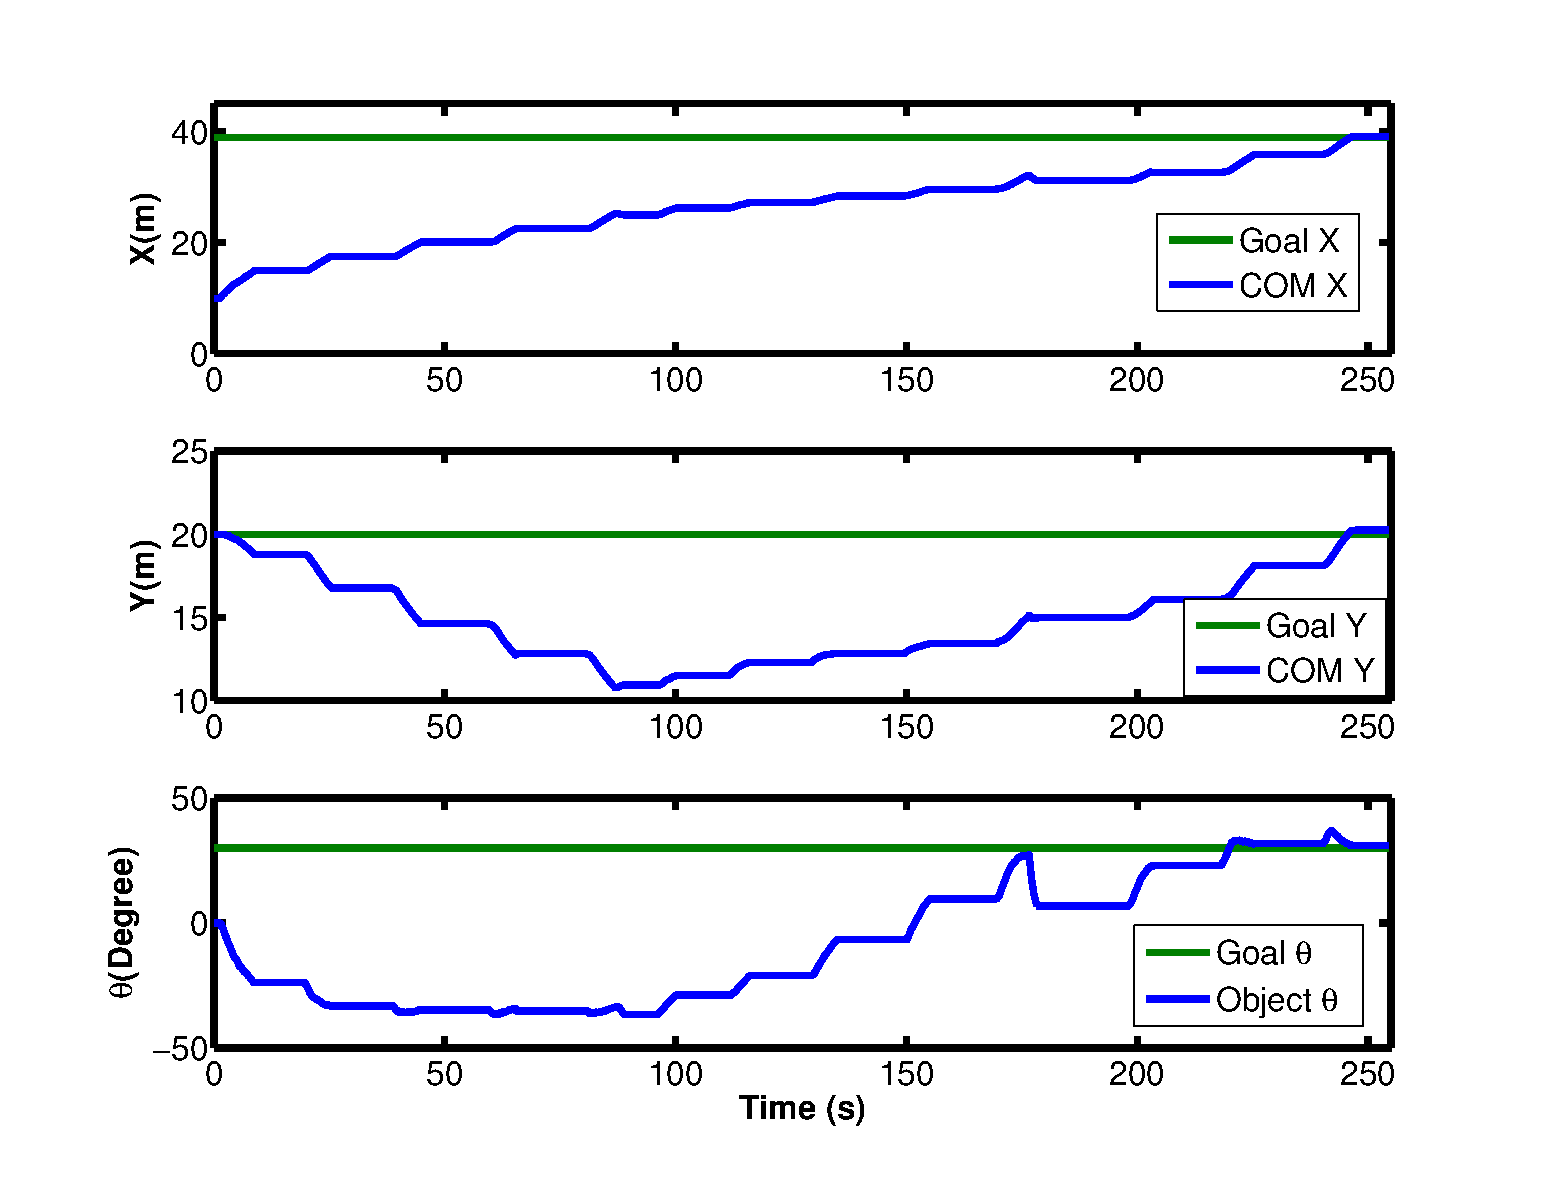
\includegraphics[width=1.07\columnwidth]{PosControl.eps}
\end{center}
\vspace{-2em}
\caption{\label{fig:PosControlFig}
By using this algorithm, we can reach the goal position and orientation. The parts that the position including orientation is not changing, the swarm is in variance control mode to avoid splitting as much as it is possible. 
}
\vspace{-1em}
\end{figure}


